% !TEX root = ../main.tex

% 中英标题：\chapter{中文标题}[英文标题]
\chapter{绪论}[Introduction]

\section{本文背景及研究的目的和意义}[Background, objective and significance of the subject]
近年来，随着互联网的快速发展和数据规模的急剧膨胀，现实世界的信息量呈现出指数级增长的趋势。用户在享受信息便利的同时，也面临着“信息过载”的问题，即如何在海量数据中高效地筛选出符合个人兴趣和需求的内容，已成为当前研究和产业界的核心挑战之一。推荐系统（Recommender System, RS）正是在这一背景下应运而生，它通过分析用户与物品之间的历史交互关系来学习用户与物品的表示，从而为用户提供个性化的内容推荐\cite{中文推荐算法综述2009, gao2022graph-survey,zhou2023comprehensive}。推荐系统如今已成为互联网产品的重要组成部分，被广泛应用于视频播放平台（如YouTube、抖音）、音乐平台（如QQ音乐、网易云音乐）以及电子商务平台（如淘宝、拼多多、京东）等，在为用户提供更好体验的同时，也为企业带来了显著的商业收益。

推荐系统的发展大致经历了从基于相似度的协同过滤（Collaborative Filtering, CF）\cite{collaboratives2025survey}，到基于深度学习的表示学习方法\cite{zhou2023comprehensive}，再到近年来基于图神经网络（Graph Neural Network, GNN）\cite{gao2022graph-survey}的阶段。协同过滤通过度量用户或物品间的相似性实现推荐，而深度学习方法利用神经网络提升了特征表示能力。近年来，GNN被广泛应用于推荐系统中，能够在用户–物品二部图上建模高阶关系，通过消息传递机制（message passing）捕捉潜在的交互模式，从而显著提升推荐性能。

然而，现有的大多数图神经网络推荐方法仅基于用户的单一目标行为（如购买）进行建模\cite{he2020lightgcn, fan2023graphDA, wang2019NGCF}，这种简化假设在实际应用中存在显著局限性。在真实的互联网场景中，用户往往会对同一物品产生多种行为\cite{chen2021GHCF, gu2022S-MBRec}，例如浏览、收藏、加购、购买等，这些行为不仅反映了用户对物品的不同兴趣强度，也蕴含了更丰富的意图语义。为了解决数据稀疏问题并使推荐模型更贴近实际场景，研究者提出了多行为推荐系统（Multi-Behavior Recommendation, MBR），通过引入辅助行为来扩充目标行为的交互，从而在一定程度上提升了模型的表达能力与泛化性能。

但与此同时，引入辅助行为虽然能够丰富交互信号，但同时也带来了新的挑战。由于辅助行为的获取成本远低于目标行为，这些交互中不可避免地包含大量噪声行为，即与用户真实兴趣不一致或无效的交互信息。如果直接将这些噪声数据用于建模，可能会干扰模型学习用户的真实偏好，导致推荐结果的准确性下降。因此，如何在多行为推荐中有效识别并抑制噪声行为的影响，成为该领域亟待解决的重要问题。

针对目前多行为推荐去噪研究的不足，本文拟提出一种基于图神经网络的多行为去噪推荐模型，通过在多行为图结构中引入噪声建模与关系加权机制，实现对多源行为的联合学习与鲁棒推荐。该研究有助于提升推荐系统在复杂行为场景下的准确性与鲁棒性，并为多行为数据的统一建模与泛化能力提升提供新的思路，对推动推荐系统在真实环境中的稳定性与应用效果具有重要意义。

\section{国内外相关研究概述}


\subsection{基于图神经网络的推荐算法研究现状}
近年来，图神经网络凭借其在处理图结构化数据方面的强大建模能力，已成为推荐系统领域的重要研究方向。推荐系统的核心任务是基于用户的历史行为预测其未来的兴趣偏好，而用户与物品之间的交互关系可以自然地建模为图结构，这使得 GNN 在该场景中展现出独特优势。

GNN 能够在用户–物品二部图上建模高阶交互关系\cite{ying2018Pinsage}。其中，用户和物品分别作为节点，交互行为作为边，通过消息传递与聚合机制，模型能够捕获潜在的关系模式，从而学习到更具表达力的用户与物品表示。此外，GNN 还可进一步融合外部信息，例如用户的社交关系\cite{wu2019Social} 和物品的知识图谱\cite{wang2019Knowlegde-Graph}，以构建统一的表示学习框架，更全面地刻画推荐系统中的异构数据特征。

2019 年，Wang 等人提出 NGCF模型\cite{wang2019NGCF}，首次将协同过滤信号引入图神经网络的消息传递过程中。模型通过多层邻居信息聚合捕获用户与物品之间的高阶关系，从而学习到更加丰富的特征表示。然而，由于引入非线性变换和多层传播，NGCF 的计算复杂度较高，并容易出现过度平滑（over-smoothing）问题。

2020 年，He 等人提出 LightGCN模型\cite{he2020lightgcn}，在结构上对 NGCF 进行了简化。该模型去除了非线性激活函数和特征变换，仅保留邻居聚合与层间加权操作。通过多层传播与加权融合，LightGCN 在显著降低计算复杂度的同时，仍能保持优异的推荐性能，证明了简洁的图卷积结构在推荐任务中的有效性。

随着研究的深入，学者们开始关注如何进一步提升 GNN 模型的泛化能力与鲁棒性。2021 年，Wu 等人提出 SGL模型\cite{wu2021SGL}，引入自监督对比学习机制，通过对用户–物品图进行数据增强，生成不同视角的图表示，并最小化同一节点在不同视角下的嵌入差异，从而提升模型的泛化性能。2022 年，Liu等人提出 SimGCL模型\cite{liu2024simgcl}，在 SGL 的基础上去除了复杂的数据增强操作，通过在节点嵌入中添加噪声扰动实现对比学习，以更简洁的结构获得了与 SGL 相当甚至更优的推荐效果。这些研究表明，自监督与对比学习方法能够有效增强图神经网络在推荐任务中的稳定性与泛化能力，为后续研究提供了新的方向。

综上，基于图神经网络的推荐研究已取得显著进展，但在多行为建模方面仍存在不足。为进一步挖掘用户偏好的多层次特征，研究者开始探索基于图神经网络的多行为推荐方法，这将在下一节中详细介绍。

\subsection{基于图神经网络的多行为推荐研究现状}
传统的推荐模型通常仅利用单一类型的用户–物品交互行为进行建模，因此容易面临数据稀疏和冷启动等问题。多行为推荐通过引入多种用户–物品交互类型（例如浏览、收藏、加入购物车等），为缓解上述问题提供了有效的解决思路\cite{RJXB202405021, JSJY20240626002, HNSF202304008, ZDZC202310007}。在多行为场景中，如何实现辅助行为（如浏览、收藏、加购）与目标行为（如购买）之间的有效信息融合，一直是学术界关注的研究重点。相关研究主要聚焦于探索不同行为之间的语义关联与交互机制，以提升目标行为的预测性能。图 1-1 展示了多行为推荐中典型的多种行为数据形式及其对应的推荐目标。

\begin{figure}[h]
\centering
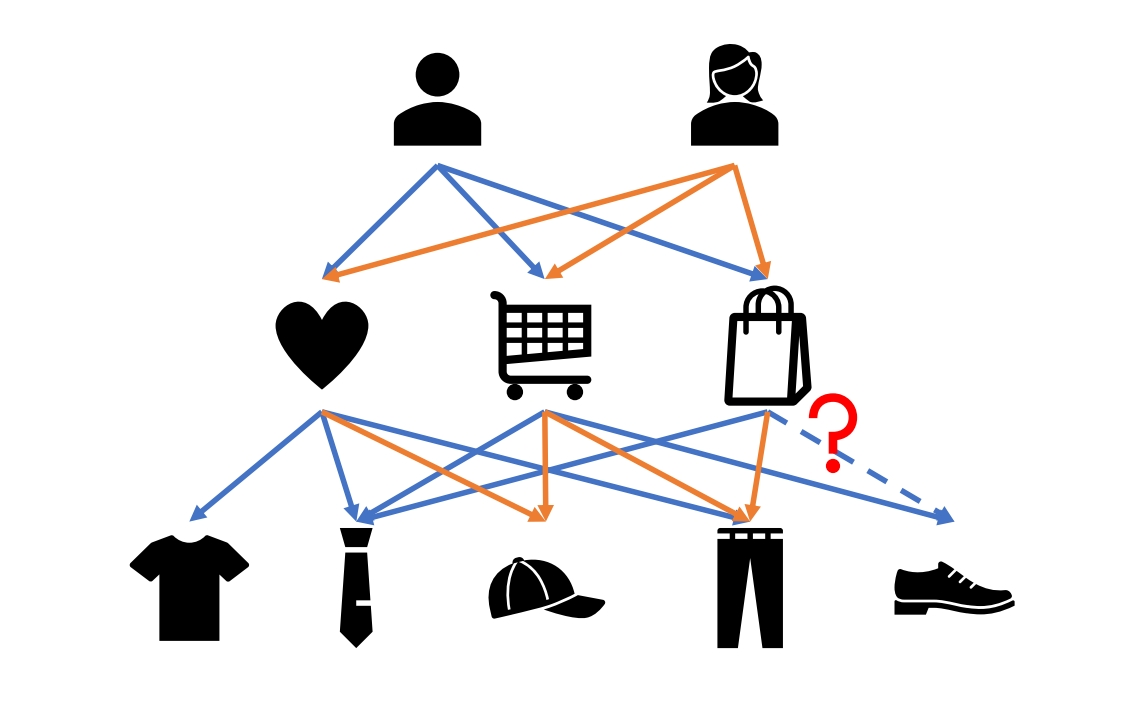
\includegraphics[width = 0.75\textwidth]{figures/Multi-Behavior-U-I.png}
\caption{多行为推荐的数据形式\cite{gao2022graph-survey}}
\label{fig:Multi-Behavior-U-I}
\end{figure}

2020 年，Jin 等人 \cite{jin2020MBGCN} 为区分不同行为的强度并融合多行为的语义信息，提出 MBGCN 模型。该方法基于多种行为数据构建统一的异构图结构，在用户–物品二部图上学习各类行为的交互贡献，并在物品–物品共同交互图上建模不同行为之间的语义相关性。模型通过在统一图中实现多层消息传递，使不同类型的行为信号能够相互补充，从而提升用户表示的准确性。最终，MBGCN 通过聚合行为贡献和语义得分生成预测结果。该模型为多行为数据的图融合提供了新的思路，但在处理噪声行为和建模行为间依赖方面仍存在局限。

2021 年，Xia 等人 \cite{xia2021MB-GMN} 指出，不同类型的用户–物品交互之间存在复杂的依赖关系，且用户行为模式差异显著。例如，一些用户仅在购买意图明确时才会收藏商品，而另一些用户可能频繁收藏但很少购买。为解决该问题，作者提出 MB-GMN模型，引入元学习框架提取跨行为知识。具体而言，MB-GMN 将不同行为视为不同的任务，通过元网络在训练过程中动态调整图神经网络的参数，以实现行为间的知识迁移。该方法不仅捕捉了多行为之间的依赖关系，还使模型在面对新的行为模式时具有更强的适应性。然而，模型的训练复杂度较高，对参数初始化和任务划分的敏感性较强。

2022 年，Gu 等人 \cite{gu2022S-MBRec} 认为早期多行为推荐研究过于强调行为差异，而忽视了行为间的潜在共性。为此，作者提出 S-MBRec模型，通过自监督学习捕捉目标行为与辅助行为之间的嵌入共性，从而缓解监督信号稀疏的问题。该模型在训练阶段构建正负样本对，通过最大化目标行为与辅助行为嵌入的一致性，提升模型对高质量信号的利用率。S-MBRec 有效减少了辅助行为冗余，提高了模型的鲁棒性，但在面对噪声较多的辅助行为时，仍缺乏显式的噪声识别机制。

2023 年，Cheng 等人 \cite{cheng2023cascading} 观察到多行为在实际应用中通常具有顺序性（如点击 → 加购 → 购买），不同行为之间存在潜在的因果依赖。基于此，作者提出 Cascading GCN 模型，设计了级联结构以显式建模行为间的层次关系。该模型将前一行为学习到的嵌入通过特征转换操作输入到下一行为的图卷积层中，从而在嵌入传播过程中保留行为依赖信息。通过这种方式，模型能够更准确地刻画用户兴趣的动态演化过程。该方法在行为序列建模方面具有较好的解释性，但对行为顺序的依赖较强，难以适应多样化的非线性行为模式。

2024 年，Zhang 等人 \cite{zhang2024POGCN} 指出，以往多数多行为推荐方法将每种行为独立建模并分别训练，导致多行为信息融合不足。为此，提出 POGCN模型，定义不同行为之间的偏序关系，并将行为组合建模为加权边，以构建统一的加权图结构。通过在该偏序图上进行图卷积操作，模型能够在保持行为层次差异的同时，实现全局的行为融合。POGCN 在捕捉行为语义结构方面取得良好效果，但仍未充分考虑各类行为间的信噪差异。

同年，Zhang 等人 \cite{zhang2023DPT} 提出 DPT模型，以预训练的方式对辅助行为中的交互进行去噪。该模型首先在多个单行为图上学习初始嵌入，通过计算交互得分来评估行为质量，并在训练阶段过滤得分较低的噪声交互。随后，模型在清洗后的交互数据上进行联合训练，从而获得更高质量的行为表示。DPT 在一定程度上缓解了噪声干扰问题，但其去噪操作独立于多行为关联结构，且未能区分不同行为的噪声比例差异，因此仍存在改进空间。

虽然多行为推荐已取得显著进展，但现有研究大多关注于如何将多种行为信息进行融合，而较少考虑辅助行为中潜在的噪声问题。在实际场景中，诸如点击、浏览、收藏等辅助行为通常成本较低、随意性较强，往往不能准确反映用户的真实兴趣或购买意图，从而引入大量噪声。尽管 DPT 模型\cite{zhang2023DPT} 尝试对辅助行为进行去噪，但其仍沿用单行为推荐中的独立去噪思路，未能充分建模多种行为之间的关联差异。事实上，不同行为对用户偏好的反映程度并不相同，其噪声比例也应具有差异。因此，如何在多行为推荐中有效识别并抑制噪声行为，成为当前研究亟待解决的问题，也促使去噪推荐逐渐成为新的研究方向。

\subsection{去噪推荐算法研究现状}
推荐系统主要依赖于隐式反馈（Implicit Feedback）来学习用户偏好。隐式反馈指用户在与系统交互过程中无需明确表达意图，系统根据用户的行为（如点击、浏览、收藏等）推断其兴趣偏好。与显式反馈（如评分或评论）相比，隐式反馈更易获取且更符合用户的真实行为特征。然而，在实际场景中，隐式反馈往往包含大量噪声样本，如误点击、随机浏览或非兴趣驱动的交互，这些噪声会干扰模型对用户真实偏好的学习，导致推荐性能下降。因此，如何识别并抑制噪声反馈，成为推荐系统研究中的重要问题\cite{JSJY2024S1014}。

2021 年，Wang 等人\cite{wang2021ADT} 通过分析常规推荐模型的训练过程，发现噪声反馈通常在早期训练阶段表现出较大的损失值。据此提出 ADT模型，在训练过程中根据每条隐式交互的损失值自适应地剔除潜在噪声交互。模型设计了两种策略：一是直接截断高损失样本，二是对高损失样本进行加权调整，从而动态降低噪声样本对整体优化的影响。该方法首次提出基于训练信号的自适应去噪思路，为后续工作提供了重要启发。

2022 年，Tian 等人\cite{tian2022learning-to-denoising} 指出，现有去噪方法在图神经网络推荐中往往忽略了噪声交互在邻域聚合中的传播效应。即使节点自身的噪声被部分消除，来自邻居的全局噪声仍可能干扰表示学习。此外，过度去噪还可能造成数据稀疏性加剧。为此，作者提出了图去噪模块与多样性保持模块：前者通过筛选更可靠的交互关系来优化图结构学习，后者通过联合去噪数据与多样性增强数据学习用户偏好，以平衡准确性与多样性。

2023 年，Fan 等人\cite{fan2023graphDA} 指出用户与物品的交互频次差异显著：交互稀疏的节点存在信息不足，而交互密集的节点则可能包含噪声。若仅依赖用户–物品矩阵而忽略用户–用户及物品–物品相关性，聚合范围也会受限。为此，提出 GraphDA 模型，通过在原始交互图上进行预训练以获得节点嵌入，再结合 Top-K 采样进行双向增强：对稀疏节点进行数据扩充，对高频节点执行去噪处理。该方法在缓解数据不平衡与噪声干扰方面均取得了良好效果。

2024 年，He 等人\cite{he2024double} 指出基于损失值的噪声识别方法（如 ADT）存在局限：损失与噪声之间的关联性并非总是稳定，困难样本可能与噪声样本同时被误判，从而造成信息丢失。针对这一问题，作者提出 DCF模型，通过扩展观察区间并聚合多个训练迭代中的损失值，来稳定样本评估结果。与传统的直接丢弃噪声样本不同，DCF 将被标记的噪声样本重新标注并引入训练，使模型在保持鲁棒性的同时避免了训练样本的浪费。

2024 年，Zhang等人提出 DeMBR模型\cite{zhang2025dembr}。该模型采用双层去噪机制：硬去噪通过计算多行为下用户与物品嵌入相似度并剔除低得分交互；软去噪利用语义引导机制，以强表达行为（如购买）指导弱表达行为（如点击）消除噪声。该方法有效提升了多行为推荐性能，但依赖固定行为强度假设，缺乏自适应噪声建模能力。

综上所述，现有去噪推荐研究主要聚焦于单行为隐式反馈场景下的噪声识别与抑制，通过损失监测、自适应加权或图结构重构等手段提升模型鲁棒性。然而，在多行为推荐系统中，辅助行为（如浏览、收藏、加购）普遍存在噪声，而相关研究仍较为匮乏。当前方法往往假设所有辅助行为的噪声分布一致，忽略了不同行为在用户偏好反映上的差异性。针对这一问题，本文将从“多行为去噪”的角度出发，探索在图神经网络框架下识别并抑制辅助行为噪声的新方法，以更准确地刻画用户真实兴趣并提升多行为推荐性能。

\subsection{多模态与大模型驱动的推荐研究现状}

\textbf{(1)多模态推荐研究现状}

近年来，研究者开始探索在推荐系统中融合多模态信息，以更全面地理解用户兴趣与物品语义。多模态推荐通过结合文本、图像、音频等内容特征，能够在冷启动与稀疏交互场景下显著提升模型性能。然而，现有多模态推荐方法普遍存在两个主要不足：一是多数模型仅在特征层面进行模态信息的简单融合，未能充分建模不同模态之间的交互与互补关系；二是模态特征中常存在噪声（如图像背景干扰或文本冗余描述），若未加以抑制，可能会削弱模型对用户真实偏好的刻画精度。

2021 年，Zhang 等人提出LATTICE模型\cite{zhang2021mining}，指出多模态推荐中除用户–物品交互关系外，还存在基于模态内容的隐式物品–物品关联。该方法为每种模态（如图像、文本）构建物品–物品图，并将各模态图聚合为统一的潜在结构图，在此基础上进行图卷积传播以学习高阶语义关系。该模型有效融合了模态内容与协同信号，但未显式建模不同模态间的相关性，同时忽视了模态特征中潜在的噪声干扰。

2023 年，Zhou 等人进一步提出FREEDOM模型\cite{zhou2023tale}，在 LATTICE 的基础上优化了多模态图的鲁棒性与效率。该模型通过冻结物品–物品图以减少训练开销，并对用户–物品图进行剪枝与去噪，从而抑制交互噪声带来的影响。尽管 FREEDOM 在模型稳定性与性能上表现出色，但仍未考虑不同模态之间的互补关系，也未对模态内部的噪声特征进行显式建模与抑制。

2024 年，Mo 等人提出 MGNM模型\cite{mo2024multimodal}，旨在解决多模态推荐中图神经网络层叠带来的特征冗余与模态噪声问题。该模型从局部与全局两个层面进行建模：在局部交互阶段，引入动态去冗余损失，通过特征矩阵与系数矩阵的乘积约束减少多层传播造成的特征冗余；在全局交互阶段，为每种模态设计模态引导特征去噪模块，以消除与用户偏好无关的模态噪声并捕获模态内部复杂关系。

总体而言，现有多模态推荐研究在提升模型表达能力和缓解数据稀疏方面取得了显著进展。然而，大多数方法仍主要关注模态内部特征的融合，而缺乏对不同模态间交互与语义互补关系的系统建模。同时，模态特征本身往往存在噪声与冗余信息，若未有效抑制，可能导致推荐结果偏离用户真实偏好。这些局限性为后续将大模型（LLMs）引入推荐系统以实现跨模态语义理解与知识增强提供了新的研究方向。

\textbf{(2)大模型结合推荐研究现状}

近年来，大语言模型（Large Language Models, LLMs）在自然语言处理领域展现出强大的语义理解与推理能力，推动了推荐系统研究的新方向。LLM 在推荐系统中的应用主要集中于特征工程阶段，利用其开放世界知识与逻辑推理能力对原始数据进行后加工与数据增强，以生成语义更丰富的特征或样本，缓解数据稀疏与冷启动问题。然而，现有多模态推荐方法往往忽视模态之间的关联性与模态内部的噪声特征，导致特征融合效果受限。为此，本文引入大语言模型作为语义引导模块，通过深层语义建模与关系补全来显式建模模态间关联，并削弱模态内部噪声，从而实现跨模态信息的语义对齐与高质量特征融合，提升推荐系统的鲁棒性与语义表达能力。

2024 年，Wei 等人提出了 LLMRec 模型 \cite{wei2024llmrec}，该方法充分利用LLM在知识建模与逻辑推理方面的强大能力，从自然语言视角对推荐图进行增强，以缓解推荐系统中普遍存在的数据稀疏与低质量侧信息问题。具体而言，LLMRec 设计了三种基于 LLM 的图增强策略：强化用户–物品交互边以丰富隐式反馈信号、增强物品节点的语义理解以提升内容表示能力，以及构建基于自然语言的用户画像以改进个性化建模。

2024年，Xu 等人 \cite{MMPOI} 针对兴趣点推荐中数据稀疏的问题，引入了多模态内容信息（如文本与图像）以增强模型的语义表达能力。该方法采用统一的预训练模型，从不同模态中提取对应的语义特征，从而缓解了模态间的语义不一致问题。具体而言，MMPOI 首先利用预训练的图文生成模型 BLIP2 \cite{BLIP-2} 将图像内容转化为文本描述，再通过统一的预训练语言模型 Sentence-BERT \cite{Sentence-BERT} 提取各模态的语义表示，实现视觉与文本模态语义空间的对齐与融合。

2025 年，Wang 等人提出了 LLaRD 模型 \cite{wang2025unleashing}，指出现有推荐系统去噪方法主要依赖外部知识或交互数据学习策略，但前者受限于知识可用性，后者往往依赖固定假设，难以准确识别复杂场景下的噪声。为此，LLaRD 利用大型语言模型（LLM）的知识与推理能力，引入语言先验以提升去噪效果。该模型首先通过 LLM 从观测数据中提取语义与偏好知识，然后结合链式思维CoT推理挖掘用户–物品关系，从而识别并过滤无关或错误交互。

总体来看，近年来大语言模型（LLMs）在推荐系统中的引入，为缓解数据稀疏、语义不一致及噪声干扰等长期难题提供了新的思路。相关研究表明，LLM 不仅能够利用其开放世界知识和推理能力丰富用户与物品的语义表示，还能在多模态融合与交互建模中发挥语义引导作用。

\subsection{研究概述小结}
在多行为推荐系统中，现有研究主要聚焦于利用多种用户交互行为（如点击、加购、收藏和购买）来缓解数据稀疏问题并提升推荐精度。然而，尽管多行为建模显著改善了用户偏好的捕获能力，现有方法在噪声识别与偏好提取方面仍存在若干不足与挑战：

\begin{enumerate}[label={(\alph*)}]
    \item \textbf{辅助行为噪声问题：} 辅助行为虽能提供额外的用户偏好线索，但其中包含大量与真实兴趣无关的交互，例如偶然点击或临时操作。这些噪声会在图传播过程中被放大，导致模型学习到的用户偏好偏离真实分布。目前大多方法仍将不同辅助行为视为等价信号，缺乏对行为强度差异与行为内相关性的细粒度建模。

    \item \textbf{行为间依赖关系建模不足：} 多行为推荐往往将辅助行为直接与目标行为进行融合，却忽略了行为间的层次与依赖结构。例如，加购行为对购买的促进作用远强于点击行为，若未能显式区分不同行为的影响强度，容易引入跨行为噪声并造成信息混淆。

    \item \textbf{模态特征噪声与异构性问题：} 随着多模态推荐的兴起，视觉、文本等模态特征被广泛用于丰富物品表示。然而，不同模态间存在显著的语义空间差异，而单一模态内部也常含有噪声或冗余信息。若缺乏有效的模态对齐与噪声抑制机制，模态融合反而可能削弱推荐的语义一致性。

    \item \textbf{语义层面真实偏好提取不足：} 当前大多数方法仅依赖结构化交互数据进行建模，忽视了从语义层面理解与提炼用户真实偏好的可能性。由于交互行为背后潜藏着复杂的语义意图，单纯依赖协同信号难以全面刻画用户兴趣。
\end{enumerate}

综上，现有研究在多行为推荐的去噪建模中仍存在结构层与语义层的双重瓶颈。为此，本文分别从\textbf{协同信号层面与语义层面}提出系统性改进：第一，设计基于协同信号的\textbf{跨行为与行为内加权去噪机制}，结合对比学习以区分真实偏好与辅助噪声；第二，引入\textbf{大语言模型（LLM）生成的模态语义信息}，通过模态引导的\textbf{硬去噪与软去噪策略}实现跨模态语义对齐与噪声抑制，并进一步通过模态驱动的对比学习增强语义一致性，从而实现多层次、可解释的多行为去噪推荐。

\section{本文的主要研究内容及章节安排}[Main research contents of this subject]


\subsection{主要研究内容}
在信息过载与多样化交互行为日益增长的时代背景下，推荐系统正逐步从单一行为建模迈向多行为融合的深度语义理解阶段。多行为推荐系统通过融合点击、收藏、加购、购买等多种用户交互行为，有效缓解了数据稀疏问题。然而，辅助行为中普遍存在的噪声与行为间复杂的依赖关系，使得模型难以准确识别用户的真实偏好。此外，随着多模态内容的引入，模态内部的噪声与模态间的语义差异进一步加剧了推荐的不稳定性。针对上述挑战，本文以“基于图神经网络的多行为去噪推荐方法”为核心研究目标，从协同信号层面与语义建模层面展开系统研究，提出两种创新性框架，实现了多源信息融合下的多层次去噪推荐。

首先，针对辅助行为中存在的大量噪声问题，本文设计了\textbf{噪声感知与偏好提取的多行为推荐方法}。该方法以用户—物品多行为交互图为基础，通过行为间与行为内加权机制，分别从全局行为强度与局部相似交互两个层面识别噪声交互。跨行为加权模块利用因果推断方法估计各行为对目标行为的影响强度，从而为不同行为分配合理权重；行为内加权模块则依据相似用户的共同交互模式动态调整权重，以保留高可信度的偏好信号。在此基础上，提出了权重引导的去噪机制，通过设定噪声阈值自适应地过滤低权重交互，构建高质量多行为图。随后，引入偏好感知的对比学习策略，在跨行为与行为内两个层面通过正负样本构造强化用户嵌入一致性，从而实现了对用户真实偏好的高精度捕获与表达。

其次，考虑到多模态信息在描述用户偏好与物品语义中的重要作用，本文提出了\textbf{噪声感知与偏好提取的多模态多行为推荐方法}。该方法利用大语言模型在知识理解与语义推理方面的优势，通过生成用户与物品的模态描述文本，实现跨模态特征的语义对齐与扩展。随后，在模型层面引入两种互补的去噪机制：硬去噪阶段基于模态相似度计算删除显著偏离真实语义的交互；软去噪阶段在图神经网络的消息传播过程中引入模态引导的注意力机制，动态抑制语义噪声传播。为进一步提升语义一致性，本文利用模态生成的嵌入构造正负样本对，开展模态对比学习，在特征层面强化用户与物品的语义匹配关系，实现了语义驱动的去噪与偏好增强。

综上所述，本文的研究工作从“协同信号层面”与“语义建模层面”双向出发，构建了一个层次化的多行为去噪推荐体系。前者通过行为强度建模与对比学习实现结构级噪声抑制，后者依托大语言模型实现模态语义层的噪声识别与语义补全。两者相辅相成，不仅显著提升了推荐系统的鲁棒性与泛化能力，也为多行为、多模态场景下的去噪推荐提供了新的理论与方法支撑。

\subsection{论文组织结构}

本论文的整体结构安排如下：

第一章为绪论。首先介绍多行为推荐系统的研究背景与现实意义，阐述推荐系统在多样化用户交互场景下所面临的核心问题，如噪声交互、数据稀疏及模态差异等。随后，对国内外在多行为推荐、去噪推荐、多模态推荐以及大语言模型辅助推荐等领域的研究现状进行系统梳理，分析现有方法的优势与不足，并明确本文的研究目标与创新点。最后，对论文的总体结构进行概述，为后续章节的展开奠定理论与逻辑基础。

第二章为相关技术概述。主要介绍支撑本文研究的基础理论与关键技术，包括图神经网络在推荐系统中的建模原理、消息传递机制及其在多行为场景下的应用。同时，对多行为推荐的基本框架与噪声建模思路进行阐述，并简要介绍大语言模型在语义理解与知识生成方面的核心机制，为后续模型设计及语义引导去噪方法提供必要的技术支撑。

第三章提出噪声感知与偏好提取的多行为推荐方法。针对辅助行为中普遍存在的噪声问题，构建了跨行为与行为内加权去噪模块，通过因果推断建模行为强度与相似交互关系，从多层次识别并过滤异常交互。同时，引入偏好感知的跨行为与行为内对比学习机制，以多视角强化用户与物品的嵌入一致性与语义表达能力，从而有效缓解噪声干扰与数据稀疏问题，提升推荐结果的准确性与稳定性。

第四章提出噪声感知与偏好提取的多模态多行为推荐方法。该方法充分利用 LLM 的语义理解与逻辑推理能力，为用户与物品生成文本化的模态描述，实现跨模态语义空间的对齐。在此基础上，通过模态相似度计算实现硬去噪，并在图神经网络中引入注意力机制以实现软去噪，从而削弱模态噪声并保留关键偏好特征。进一步地，结合模态对比学习策略，增强不同模态间的语义一致性与特征互补性，实现高质量特征融合与鲁棒推荐效果。

\subsection{论文整体研究框架}
本研究针对多行为推荐系统在多样化用户交互场景中普遍面临的噪声干扰、数据稀疏及模态差异等问题，构建了以图神经网络为核心的多层次去噪与语义增强推荐框架。研究主要聚焦以下三个核心问题：首先，针对多行为数据中存在的大量噪声交互，提出跨行为与行为内加权去噪算法，通过因果推断估计行为强度，结合用户间相似性建模生成加权交互图，以有效区分真实偏好与噪声交互，从而提升推荐的准确性与稳定性；其次，为解决辅助行为与目标行为之间的偏好差异问题，构建偏好感知的自监督对比学习机制，在行为内与行为间两个层面进行表征增强，强化用户与物品嵌入的一致性；最后，引入大语言模型生成的语义特征，通过文本化模态描述与语义对齐机制，建模多模态信息间的关系。基于模态相似性实现硬去噪，并在图神经网络中通过注意力机制完成软去噪，进一步提升模型的鲁棒性与语义表达能力。论文通过理论创新与语义融合，形成从多行为噪声识别、偏好表征增强到多模态语义引导去噪的系统性研究框架，为多行为推荐系统中的噪声建模与语义增强提供了新的范式，并在多个公开数据集上验证了其有效性与可扩展性。

在本研究中，第三章提出的\textbf{噪声感知与偏好提取的多行为推荐方法}，以及第四章提出的\textbf{噪声感知与偏好提取的多模态多行为推荐方法}，从不同层面为多行为推荐系统中的噪声抑制与偏好建模提供了解决方案。

第三章聚焦于多行为数据的结构与信号建模，通过构建跨行为与行为内加权去噪模块，结合因果推断与自监督对比学习，识别辅助行为中的噪声并提取真实偏好信号，形成纯净且高质量的交互表示。  
第四章则在此基础上引入大语言模型，通过语义生成与关系推理，扩展推荐系统的模态维度。该方法利用 LLM 生成的语义描述实现跨模态特征对齐，并在图神经网络中融合模态注意力机制，实现多模态层面的硬、软联合去噪，从而进一步提升推荐的语义解释性与泛化能力。

需要指出的是，第四章的研究在方法设计上继承并扩展了第三章的成果。第三章为多行为去噪奠定了结构性与因果性基础，而第四章则在此框架上通过引入语言语义与多模态信息实现更高层次的语义增强。两章在研究目标上相互独立、在技术逻辑上相互衔接，分别从行为信号与语义特征两个维度推进多行为推荐的去噪与增强研究。

从推荐流程的视角来看，第三章与第四章可视为并行互补的两条路径：前者侧重于基于交互结构的信号净化与偏好提取，后者则着眼于语义层面的知识建模与特征融合。两者共同构成完整的多行为去噪与语义引导推荐框架，为实现高精度、高鲁棒性的推荐提供了系统性解决思路与技术支撑。
